\chapter{Dataset selection}

\section{Alternatives}

	\subsection{Project Type}
	The dataset is the fundament of a data-science project. The quality, size and closeness to reality decide the degree to which the findings can be helpful for solving real problems. 
	In this section, a classification for data-science projects is introduced.
	
	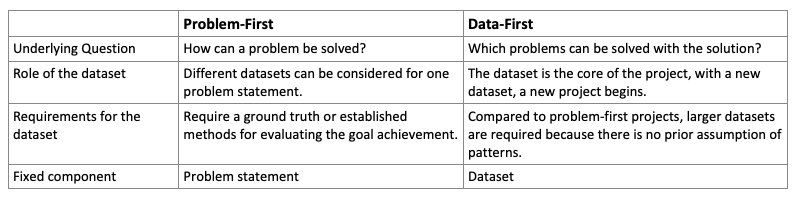
\includegraphics[height=4cm]{Bilder/meta_project.png}
	
	The problem-first project type is characterized by a predefined problem statement or research goal. The underlying question is, how a specific or a set of problems can be solved. For the selection of the dataset, this requires that goal achievement can be measured with existing ground truth. In some cases, also other methods such as expert judgements can be sufficient. In a problem-first project, different datasets can and should be considered.
	
	The complementary project type is the data-first project, which describes most data-mining projects. This type is characterized by a more explorative approach, and the goal to find problems and patterns. Here, the dataset is at the core of the project and the fixed aspect of a project. In turn, this means swapping the dataset is the start of a new project.
	
	With the project type as a decisive factor for the dataset explained, the other evaluation criteria for the dataset is described. In the corporate environment two fundamental sources for data exist. 
	
	\subsection{Data Source}
	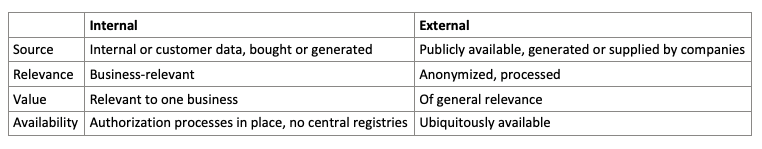
\includegraphics[height=3cm]{Bilder/internal_external.png}
	
	Firstly, data can be sourced from inside the company. This can include customer data or data generated from observation and monitoring processes inside the company. Data is either directly or very closely related to the company's business. Depending on the solution, it can be of use to customers or it can be utilized inside the company. Internally sourced data is almost exclusively rated confidential, limiting even intra-company access to it. Authorization processes and more than often not existing registries for data may hinder project progress.
	
	Secondly, data can be sourced outside the company. A vast number of online registries for data exist, both with paid and free of charge service offerings. Data sources include real-life data and data generated for educational purposes. Because of its publication, the data is stripped from all parts which could expose confidential information such as corporate secrets. Additionally, data is anonymized and processed to limit the usefulness to potential competitors.
	
	It can be stated, that both sources are suited for different goals. 